\section{Stratifying $\RR$}
\label{section:smooth-decompose}

Let $f:M\to\RR$ be a stratifying map with singular values $X_f$.
We fit closed neighbourhoods (\emph{sleeves}) around the singular values of $f$ and classify these sleeves by the maximum codimension (with respect to $\RR$) of singular values they contain.
Because $X_f$ consists of codimension 1 and codimension 2 singular values (arcs and arc-crossings respectively) in the plane and the endpoints of each arc of codimension 1 singular values is a pair of (not necessarily distinct) codimension 2 singular values,  we stratify $\RR$ into face regions that contain no singular values, edge regions that contain only codimension 1 singular values, and vertex regions, each of which contain exactly 1 codimension 2 singular value.

The naming convention is due to the natural structure $X_f$ has of an embedded planar graph whose vertices are codimension 2 singular values and whose edges are arcs of codimension 1 singular values.
We refer to the codimension 2 singularities as the vertices of $X_f$, the arcs of codimension 1 singularities as the edges of $X_f$, and the regions of regular values comprising $f(M)\setminus X_f$ as the faces of $X_f$.
Figures \ref{fig:X_f}-\ref{fig:face-sleeve} are used to illustrate the stratification resulting from sleeve-fitting.

\begin{figure}[h!]
	\centering
	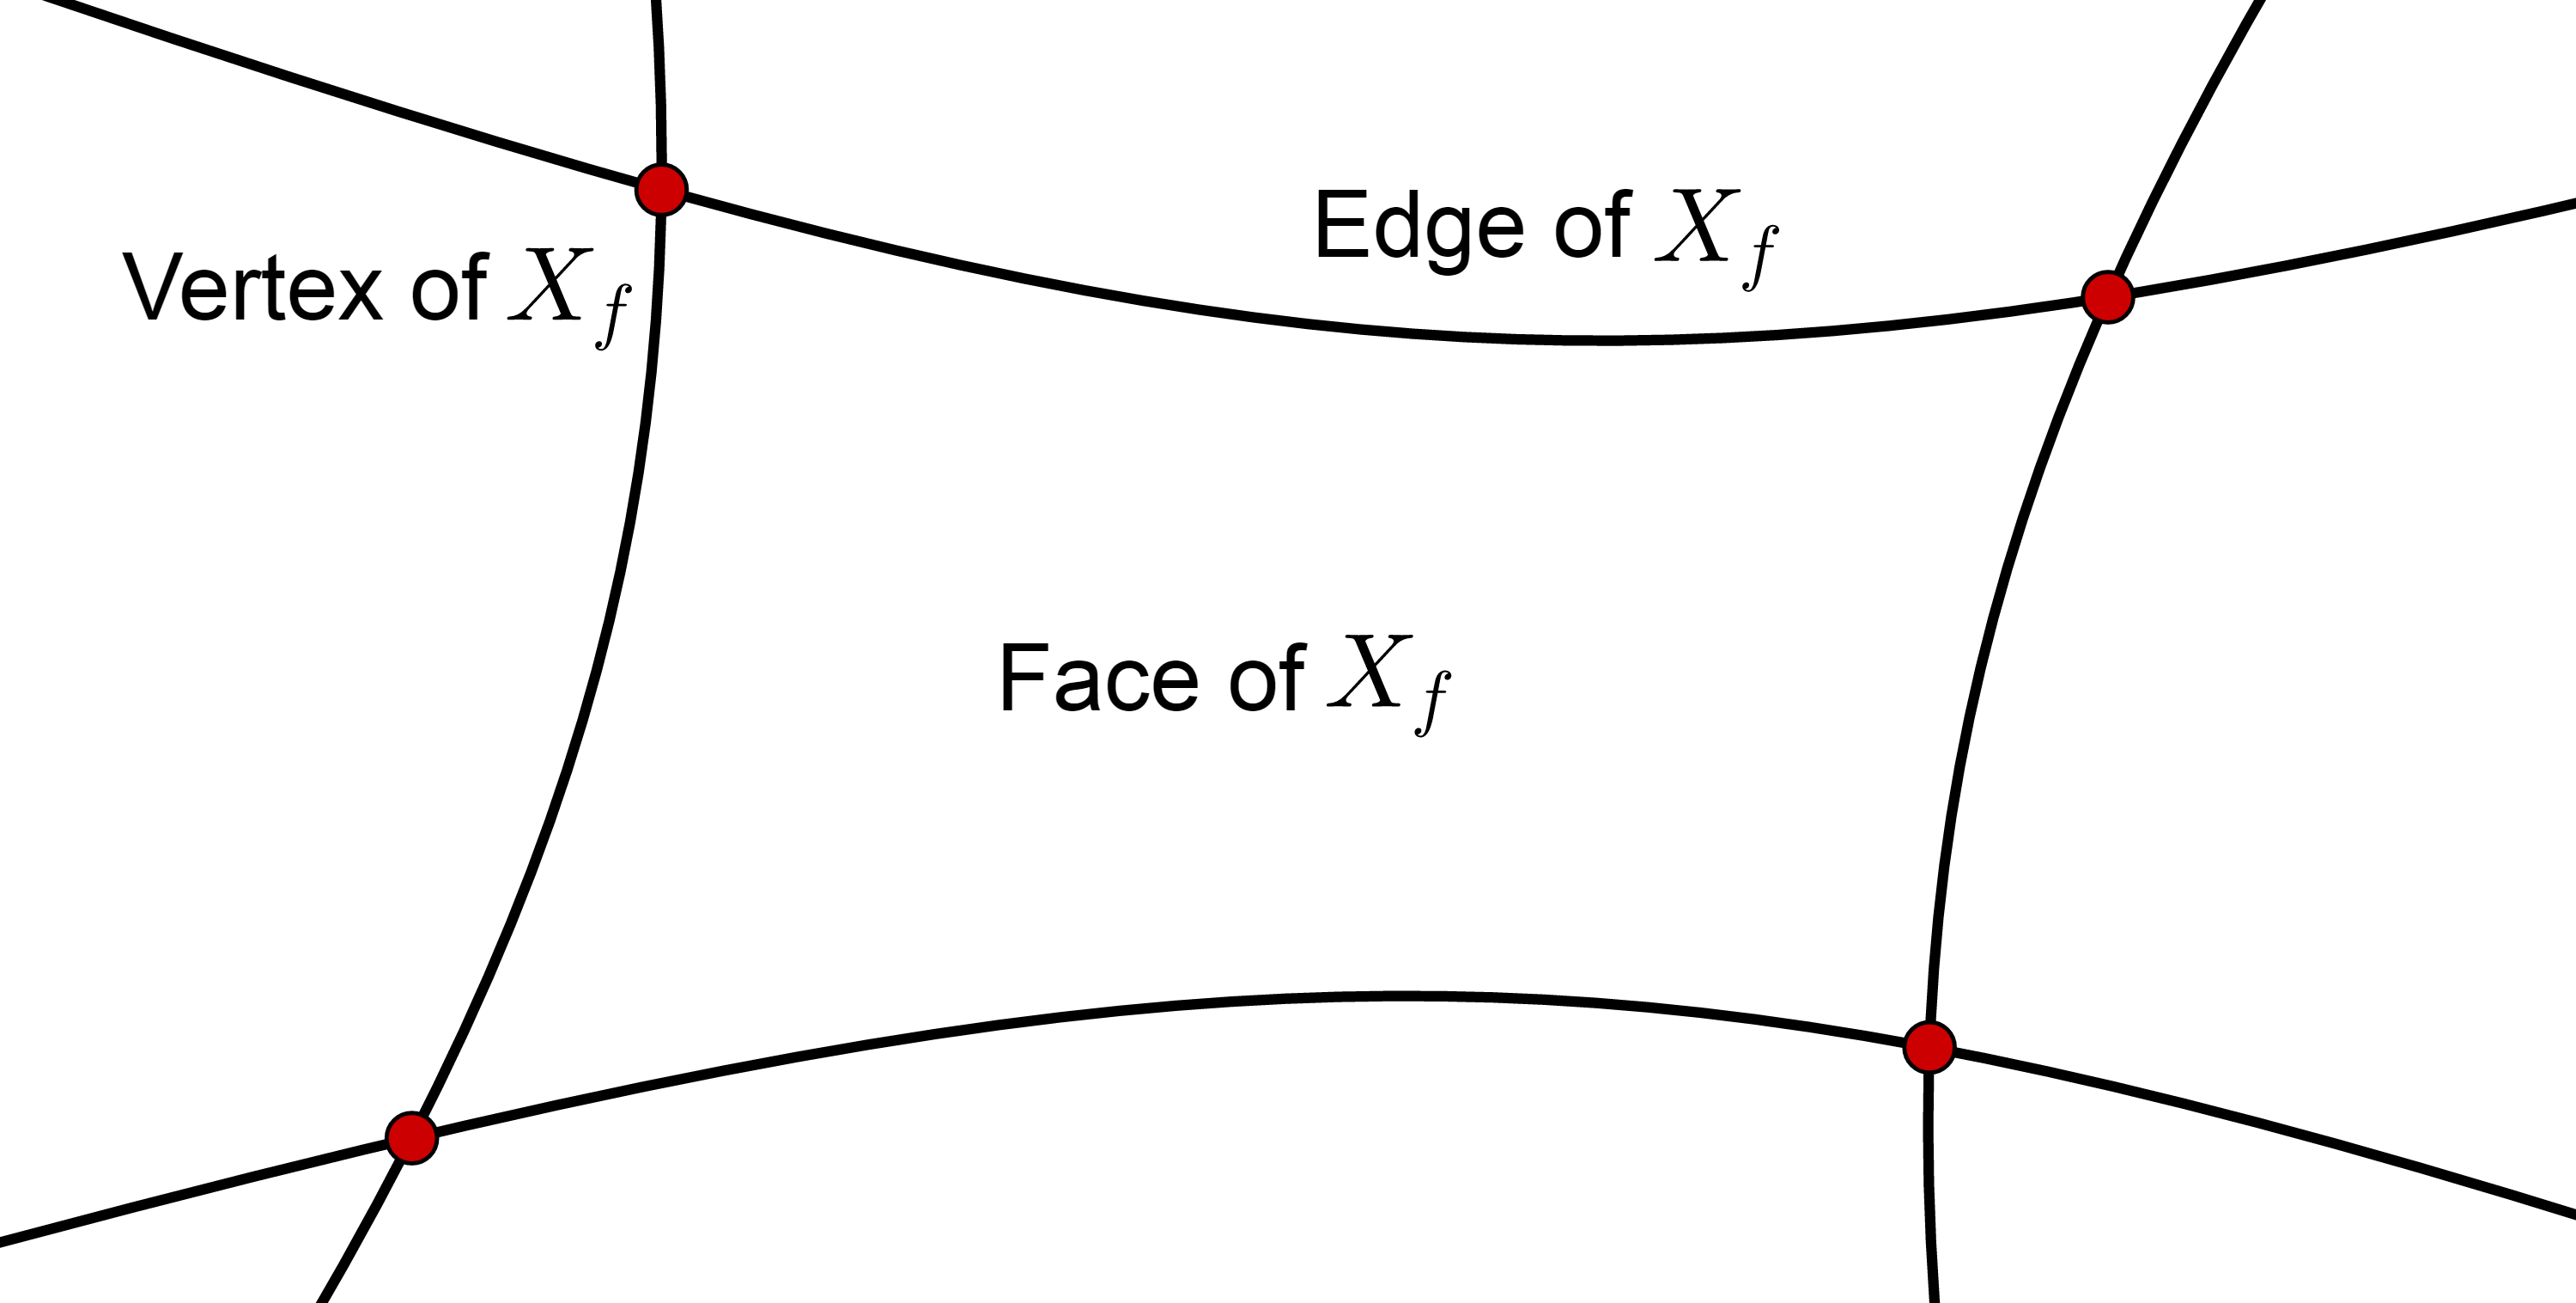
\includegraphics[width=0.7\textwidth]{figures/X_f.png}
	\caption{
		\textbf{Singular values of $f$.}
		Vertices are arc crossings, edges are arcs, and connected components of $f(M)\setminus X_f$ are faces.
	}
	\label{fig:X_f}
\end{figure}

\begin{figure}[h!]
	\centering
	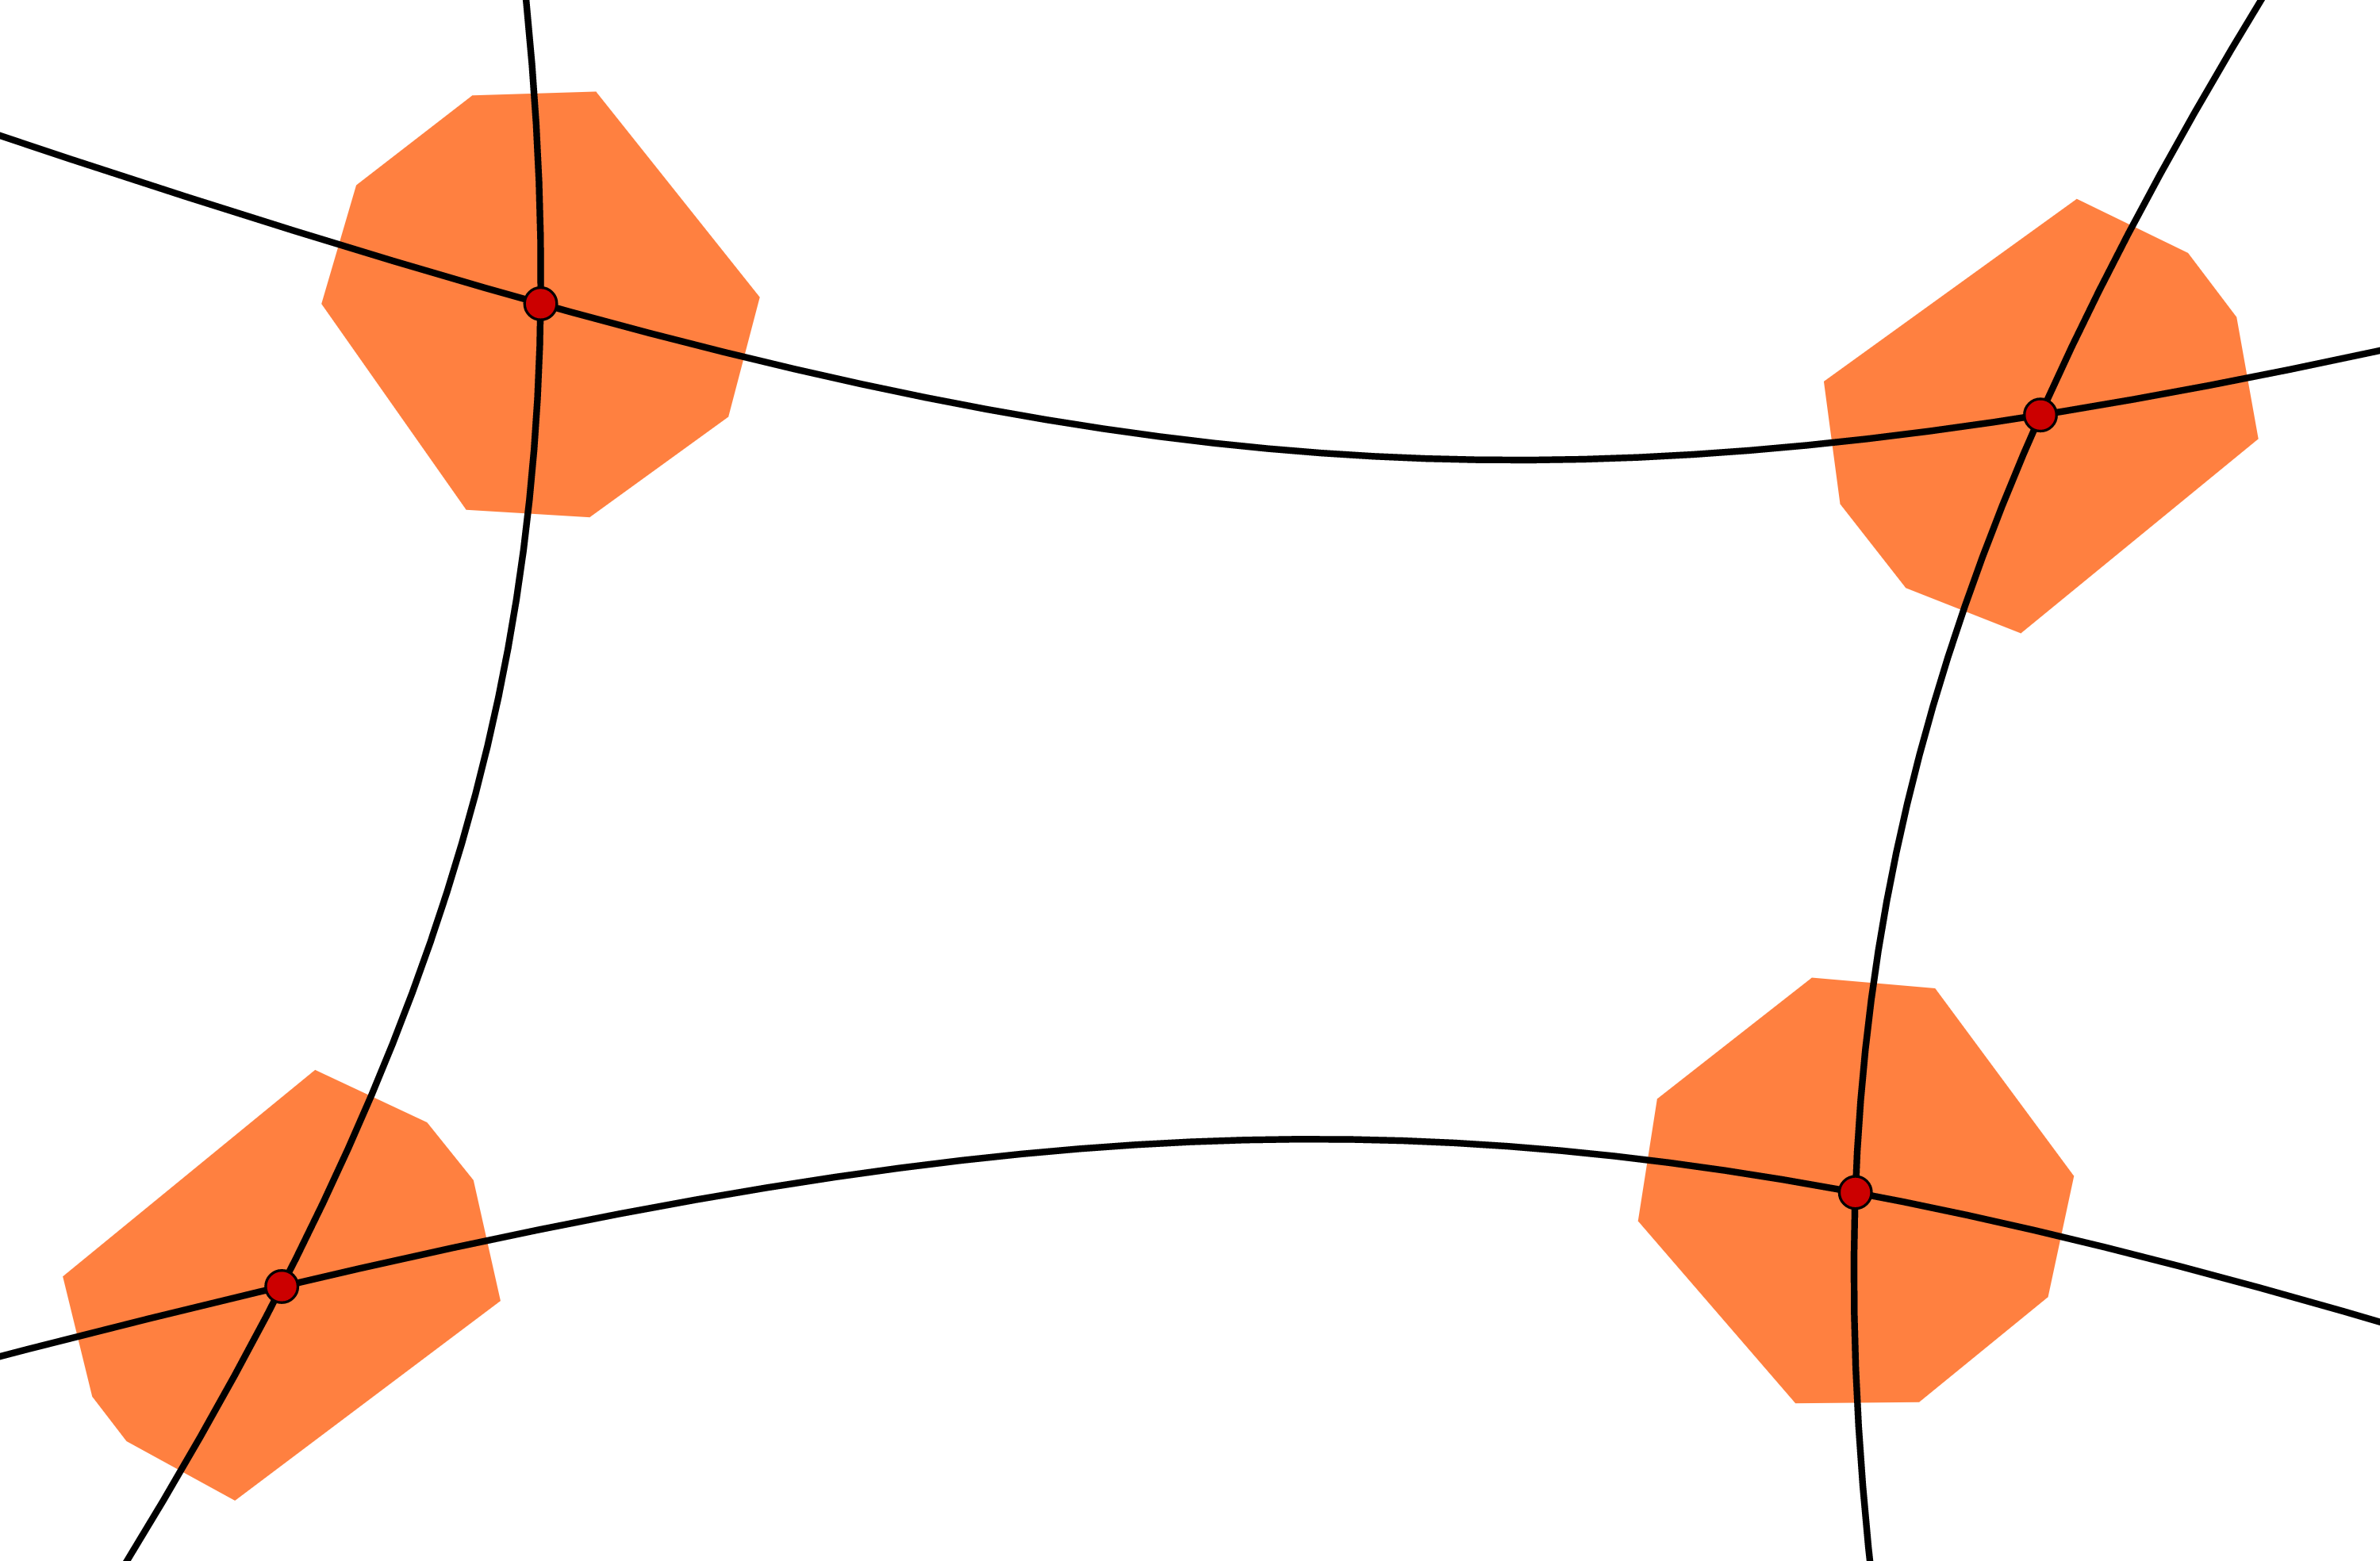
\includegraphics[width=0.9\textwidth]{figures/vertex-sleeve.png}
	\caption{
		\textbf{Forming vertex regions.}
		Octagonal sleeves are fit around the vertices of $X_f$ to form vertex regions.
		Note that the 1--strata vertex sleeves alternate between containing exactly one singular value, its intersection with an edge of $X_f$, or consisting entirely of regular values.
		New vertex regions are shaded orange.
	}
	\label{fig:vertex-sleeve}
\end{figure}

We begin by fitting sleeves around codimension 2 singular values as in Figure \ref{fig:vertex-sleeve}.
These sleeves are each boundary-stratified 2--discs with exactly eight 1--dimensional boundary strata (i.e. octagons).
Following the notation patterns already present in this document, we call the $k$--dimensional strata of a stratified manifold the \emph{$k$--strata} of that manifold.
%Octagons are used here solely to simplify descriptions further down the line of proof.
If $x$ is a codimension 2 singular value then $x$ is the result of an arc crossing, and a small neighbourhood around an arc crossing is divided into four regions of regular values.
The octagon around $x$ is fit so that its 1--strata alternate between being fully contained in a region of regular values and orthogonally intersecting one of the arcs of singular values that creates $x$, as depicted by the example fitting in Figure \ref{fig:vertex-sleeve}.

The closed octagons form the vertex regions of the stratification of $\RR$.
The octagons are chosen to be small enough that no two vertex regions overlap and such that the 1--strata that intersect arcs of codimension 1 singular values are all the same length.

\begin{figure}[h!]
	\centering
	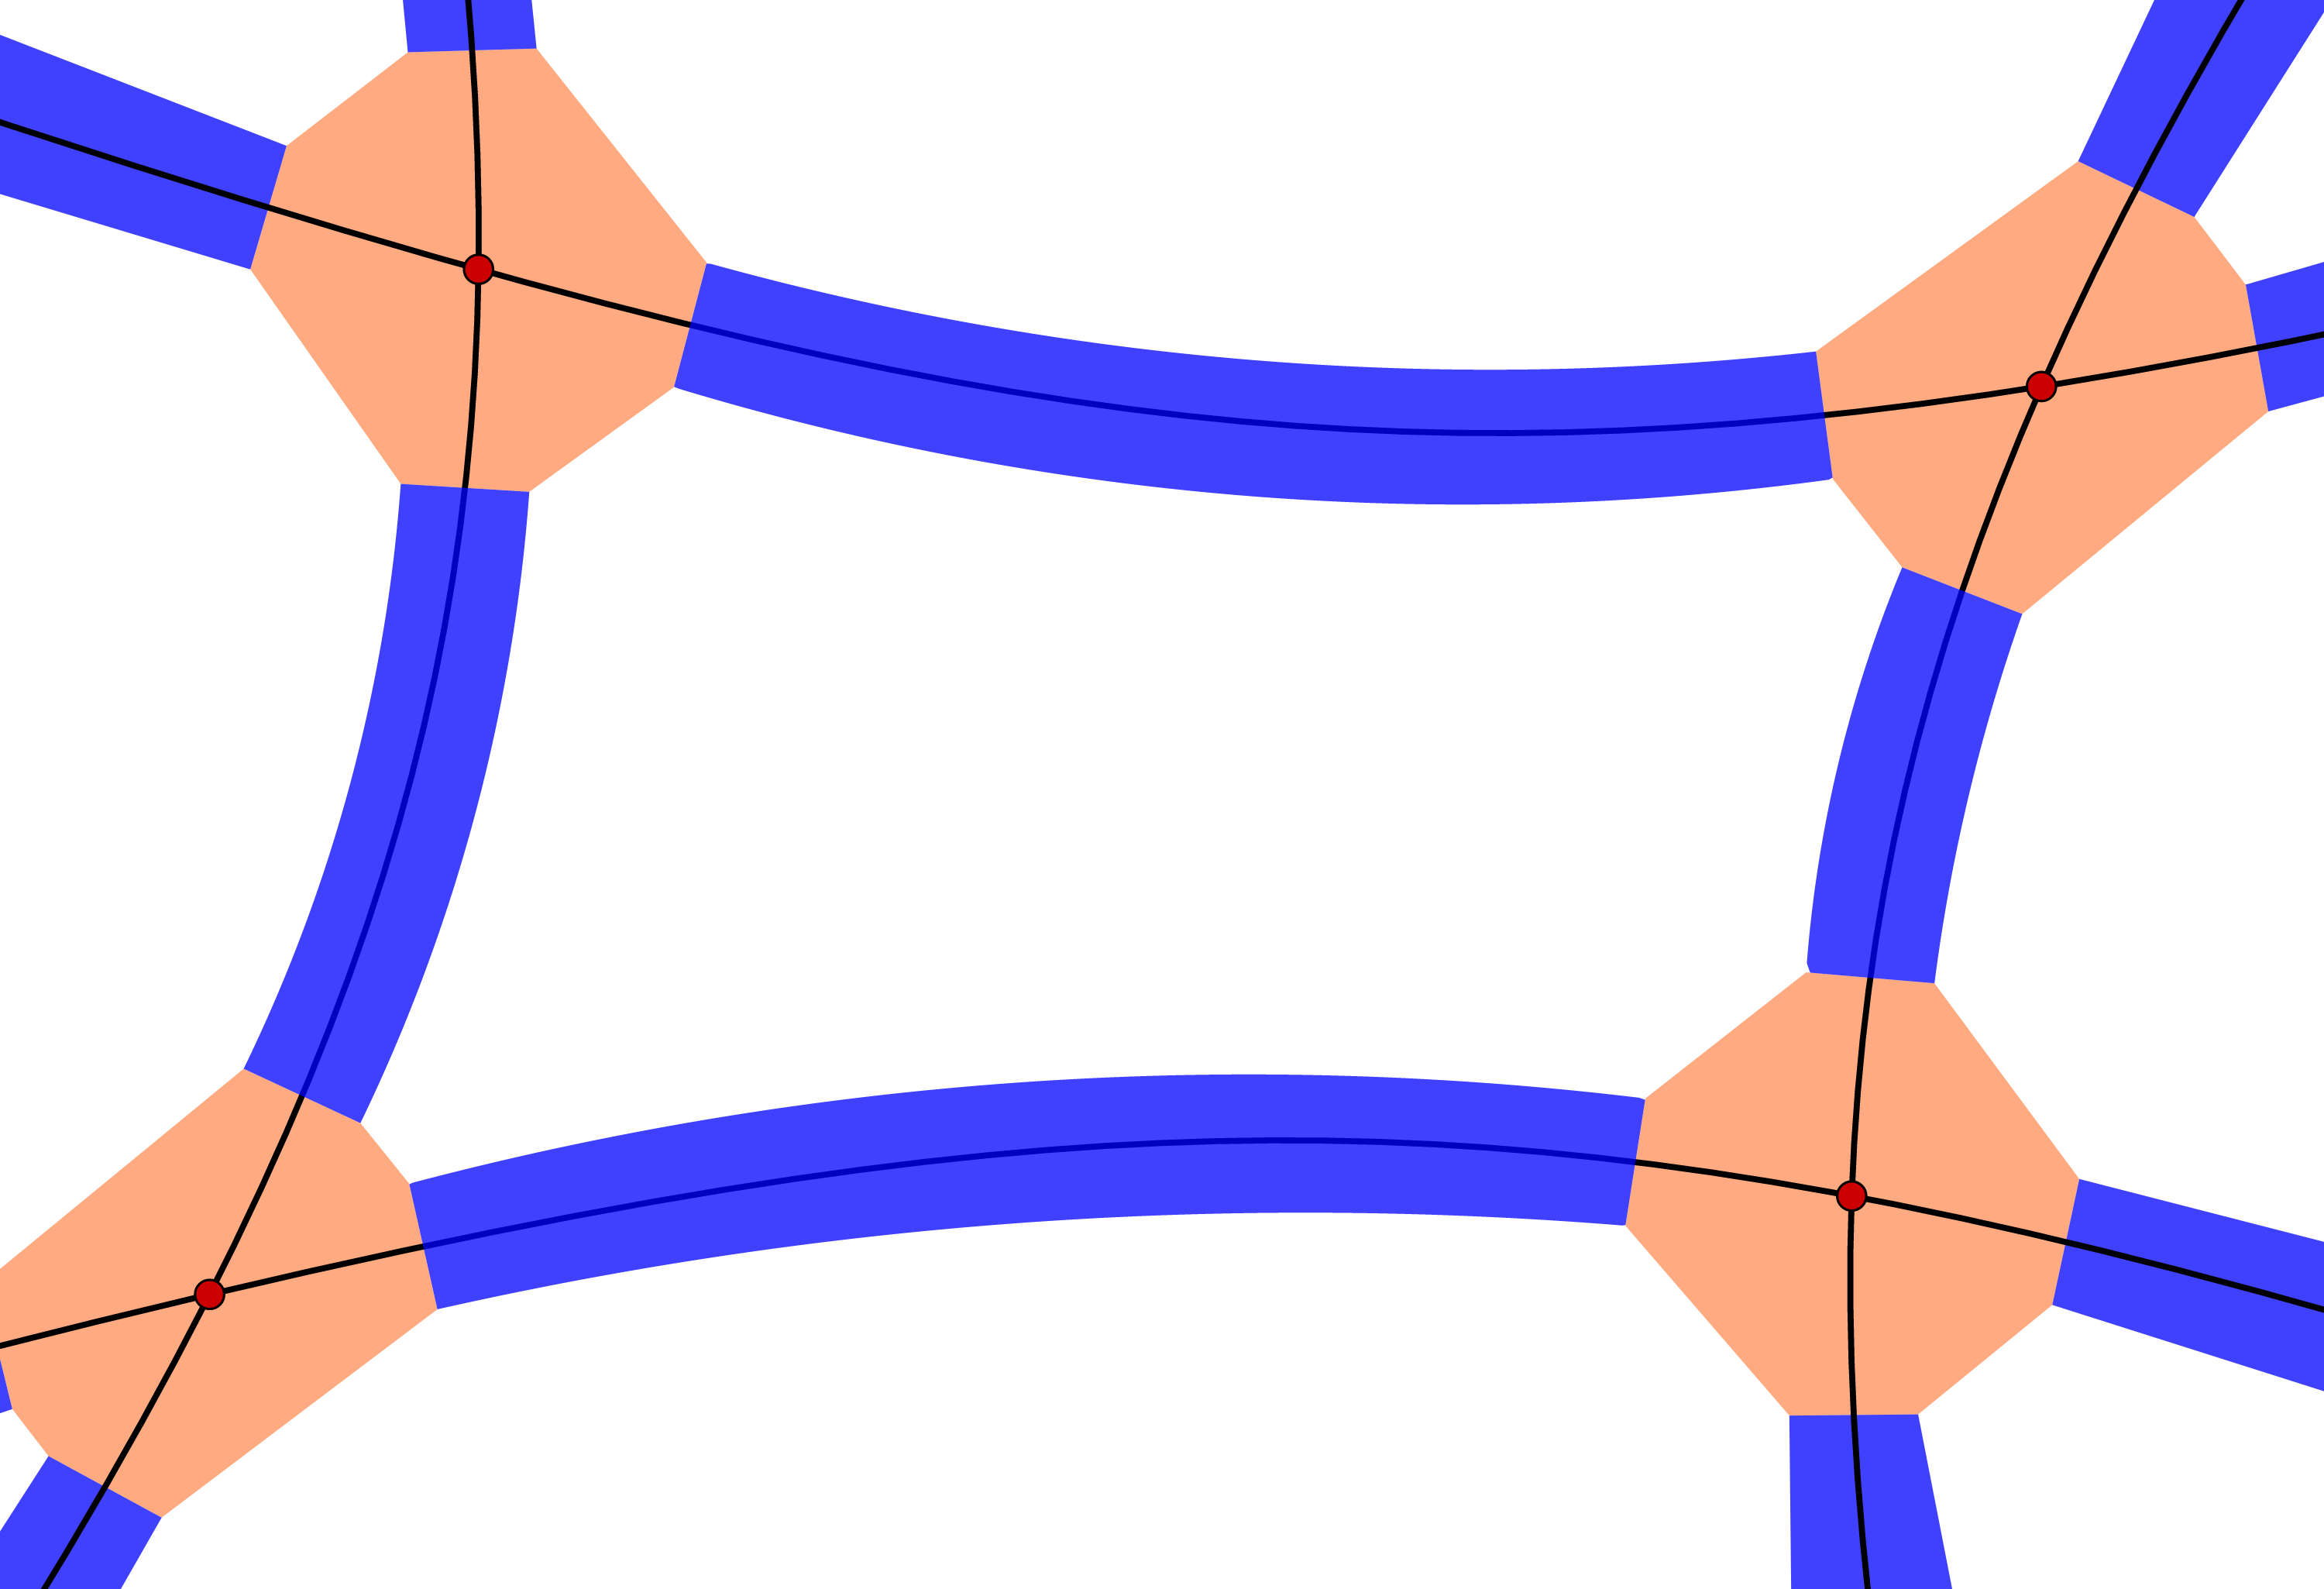
\includegraphics[width=0.9\textwidth]{figures/edge-sleeve.png}
	\caption{
		\textbf{Forming edge regions.}
		Vertex region corners are connected to fit sleeves around arcs of codimension 1 singular values to form edge regions.
		New edge regions are shaded blue.
	}
	\label{fig:edge-sleeve}
\end{figure}

Let $\gamma$ be an edge of $X_f$ with endpoints a pair of vertices.
$\gamma$ orthogonally intersects one 1--strata from each of the octagonal vertex regions fit around its endpoints, and we use these 1--strata to form the edge region associated to $\gamma$ by connecting the 0--strata boundaries of the 1--strata to one another using a pair of arcs parallel to $\gamma$, as illustrated in the example edge region fitting of Figure \ref{fig:edge-sleeve}.

We form the boundary of the edge region associated with $\gamma$ as the union of:
\begin{enumerate}
	\item the arcs parallel to $\gamma$ connecting vertex region 0--strata, and
	\item the vertex region 1--strata that intersect $\gamma$
\end{enumerate}
This union is a simple closed curve $J$.
The component of $\RR\setminus J$ that contains no vertices of $X_f$ is a boundary stratified 2--disc that shares two of its four boundary 1--strata with the vertex regions on either end of $\gamma$.
This boundary stratified 2--disc is then the edge region of the stratification of $\RR$ associated with $\gamma$.

\begin{figure}[h!]
	\centering
	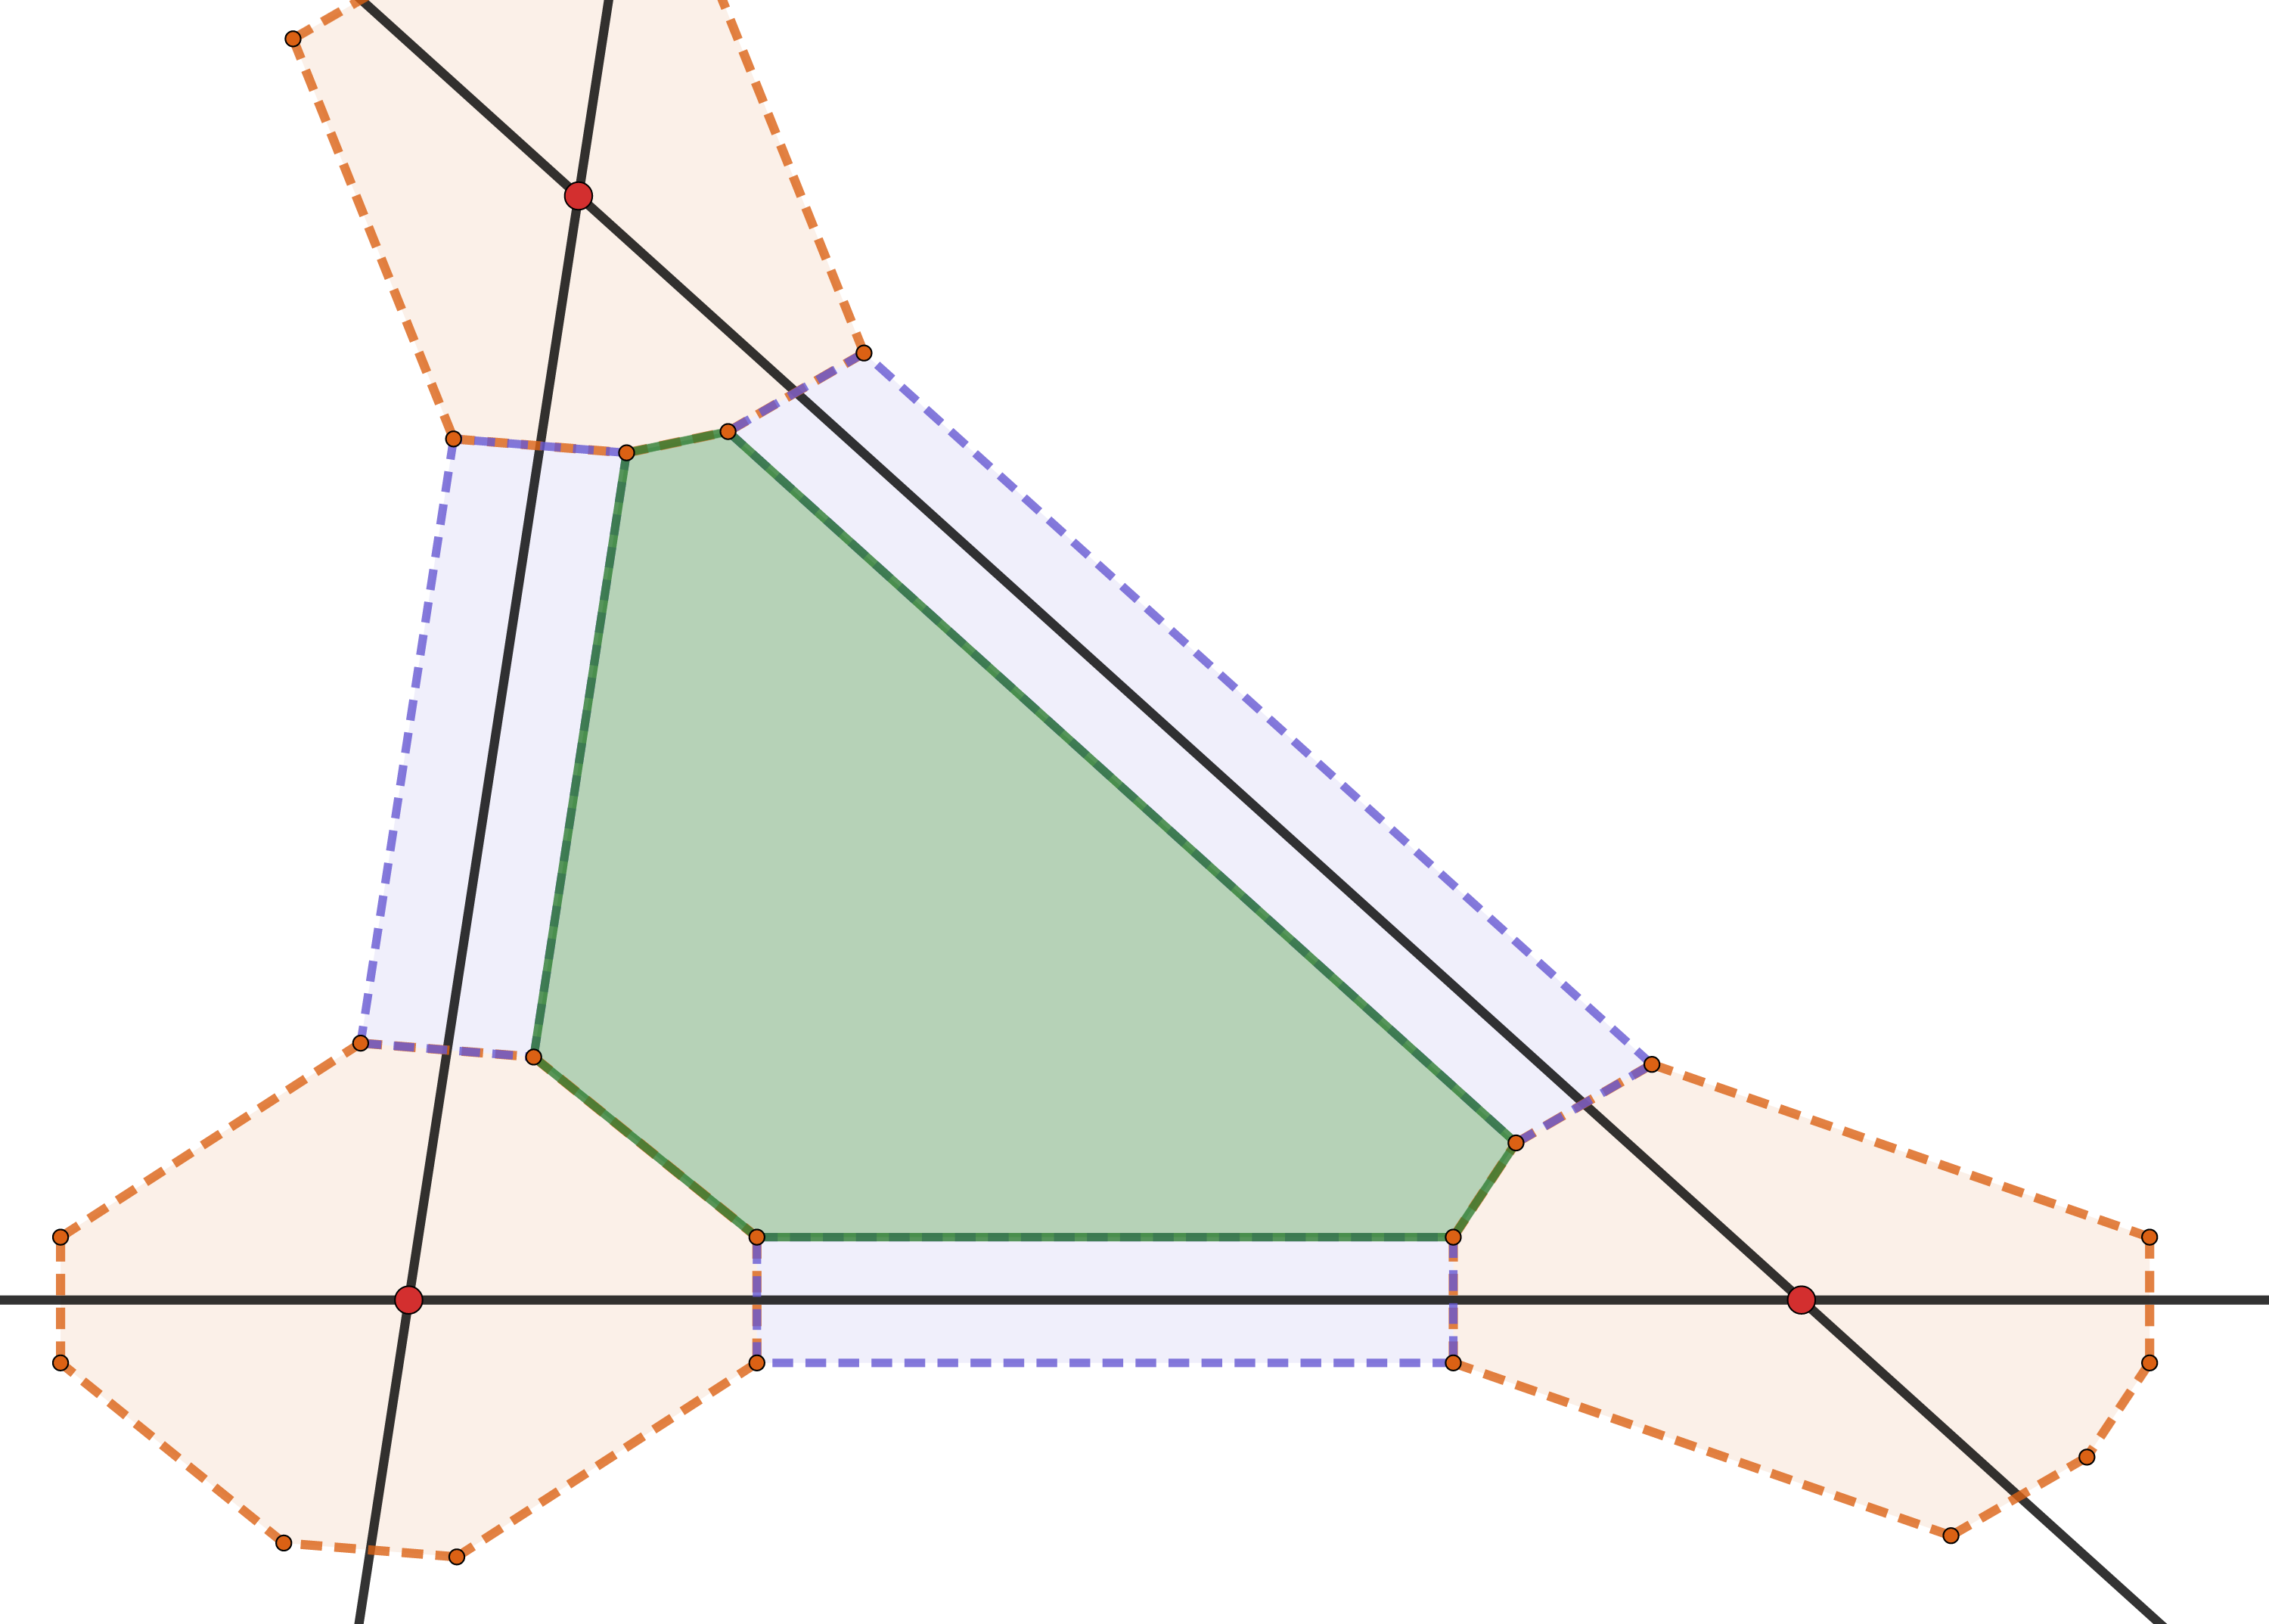
\includegraphics[width=0.9\textwidth]{figures/face-sleeve.png}
	\caption{
		\textbf{Forming face regions.}
		All remaining regions contain no singular values, and we take these to be the face regions.
		New face regions are shaded green.
	}
	\label{fig:face-sleeve}
\end{figure}

Removing from $f(M)$ all vertex and edge regions, we are left with a collection of connected regions in the plane, each of which is a deformation retract of a face of $X_f$.
%If a smooth map $f:M\to\RR$ only satisfies the first five stratification conditions then these regions need not be simply connected.
%The sixth stratification condition (that the set of singular values of $f$ in the plane is connected) guarantees that each of these region is simply connected.
%This is because the boundary components of these regions are formed by the singular values of $f$ in the plane, and different boundary components are necessarily disjoint.
%Note that a map satisfying the first five stratification conditions can be smoothly homotoped to satisfy the sixth condition, and this is argued by induction on the number of connected components of the set of singular values of $f$ in the plane.
%If $X_1$ and $X_2$ are connected components of singular values of $f$ in the plane, then let $\vec x$ be a vector such that $X_2\cup (X_1+\vec x)$ (the union of $X_2$ with $X_1$ translated by $\vec x$) is connected, and $X_2$, $(X_1 + \vec x)$ intersect transversely.
%Because $X_1 = f(\cup_i \gamma_i)$ where $\cup_i \gamma_i\subset S_1(f)$, we form a smooth homotopy of $f$ that is the identity outside of a tubular neighbourhood of $\cup_i \gamma_i$ and translation by $\vec x$ on $\cup_i \gamma_i$.
We take the closures of these to be the face regions of the stratification of $\RR$.
The boundary of each face region is an alternating collection of boundary 1--strata from edge regions and boundary 1--strata from vertex regions.
See Figure \ref{fig:face-sleeve} for an example fitting.

With all of the regions defined, we can describe precisely how $f$ stratifies $\RR$.
The stratification of $\RR$ is a stratification into subsets $R_{(i,j)}$ where $i,j$ are integers.
Subset indexing is defined so that a subset $R_{(i,j)}$ is an $i$--dimensional submanifold of $\RR$, thus $R_{(i,j)}\nleq R_{(k,l)}$ if $i\nleq k$.
The first collection of subsets used to filter $\RR$ are the 0--strata of the octagonal vertex sleeves.
We assign to these subsets the indices $(0,i)$ for $i=1\dots N_0$, where $N_0$ is the number of 0--strata.
Our 0--strata are disjoint, so for any $i,j$ with $i\neq j$, $R_{(0,i)}$ is not contained in $R_{(0,j)}$, hence $(0,i)\nleq (0,j)$.

The boundary 1--strata connect the $(0,i)$--level strata.
These 1--strata are indexed by $(1,j)$ for $j=1\dots N_1$, where $N_1$ is the number of arcs.
The boundary points of 1--strata are 0--strata and are subsets of the filtration indexed by the $(0,i)$ indices, so $(0,i)\leq (1,j)$ if and only if $R_{(0,i)}$ is one of the boundary points of $R_{(1,j)}$.
Our 1--strata intersect only at their boundary points, so $(1,j)\nleq(1,k)$ for any $j,k$. 

The regions themselves are indexed by $(2,k)$ for $k=1\dots N_2$, where $N_2$ is the number of regions.
These indices work similarly to the 1--strata indices.
The boundary of a region consists of 0-- and 1--strata, so $(n,i)\leq(2,k)$ if and only if $R_{(n,i)}$ is contained in the boundary of $R_{(2,k)}$.

With $\RR$ stratified, we move onto a stratification of $M$.
This stratification is induced by the preimages of the strata of $\RR$.

%
%Before moving on to the stratification of $M$ induced by our decomposition of $\RR$, we need to iron out the corner cases of when $X_f$ contains no codimension 2 singular values.
%
%
%Because $X_f$ is connected, $X_f=f(S_1(f))$, and $S_1(f)$ is a collection of smooth non-intersecting curves in $M$, we conclude that $S_1(f)$ contains exactly one curve.
%Furthermore, $f(M\setminus S_1(f))$ lies entirely within $X_f$ so $S_1(f)$ is everywhere a definite fold.
%
%...

